\chapter{Side Effects}
Benzodiazepines maybe addictive and overdosing may result in death. The dose and blood concentration of benzodiazepines should not be taken lightly.The two figures show the increase in the number of death of benzodiazepines with opioids \emph{Fig.}\ref{fig:op}, and the increase in the number of deaths caused by overdosing benzodiazepines \emph{Fig.}\ref{fig:bnz}.\cite{death}
\section{Chlordiazepoxide}
Chloridiazepoxide shows minimal side effects. Some side effects like: drowsiness, ataxia\footnote{the loss of full control of bodily movements.}, and confusion can be avoided by maintaining the proper dose. Syncope\footnote{temporary loss of consciousness caused by a fall in blood pressure.} has been reported at the lower  

\section{Diazepam}
The most common side effects are drowsiness, fatigue, ataxia, and muscle weakness.

The following symptoms are minor, but still reported.
\paragraph{Central Nervous System} confusion, depression, dysarthria, headache, slurred speech, tremor, vertigo

\paragraph{Gastrointestinal System} constipation, nausea, gastrointestinal disturbances
\paragraph{Special Senses} blurred vision, diplopia, dizziness
\paragraph{Cardiovascular System} hypotension
\paragraph{Psychiatric and Paradoxical Reactions} stimulation, restlessness, acute hyperexcited states, anxiety, agitation, aggressiveness, irritability, rage, hallucinations, psychoses, delusions, increased muscle spasticity, insomnia, sleep disturbances, and nightmares.
\paragraph{Urogenital System}  incontinence\footnote{lack of voluntary control over urination or defecation.}, changes in libido\footnote{sexual desire}, urinary retention


Diazepam is also subject to Schedule IV control under the Controlled Substances Act of 1970. Addiction-prone individuals (drug addicts or alcoholics) may develop physical dependence on the diazepam.

\begin{figure}
\centering
\begin{minipage}{.5\textwidth}
  \centering
  \includegraphics[width=\linewidth]{opioids.jpg}
  \captionof{figure}{The number of death with benzodiazepines with opioids}
  \label{fig:op}
\end{minipage}%
\begin{minipage}{.5\textwidth}
  \centering
  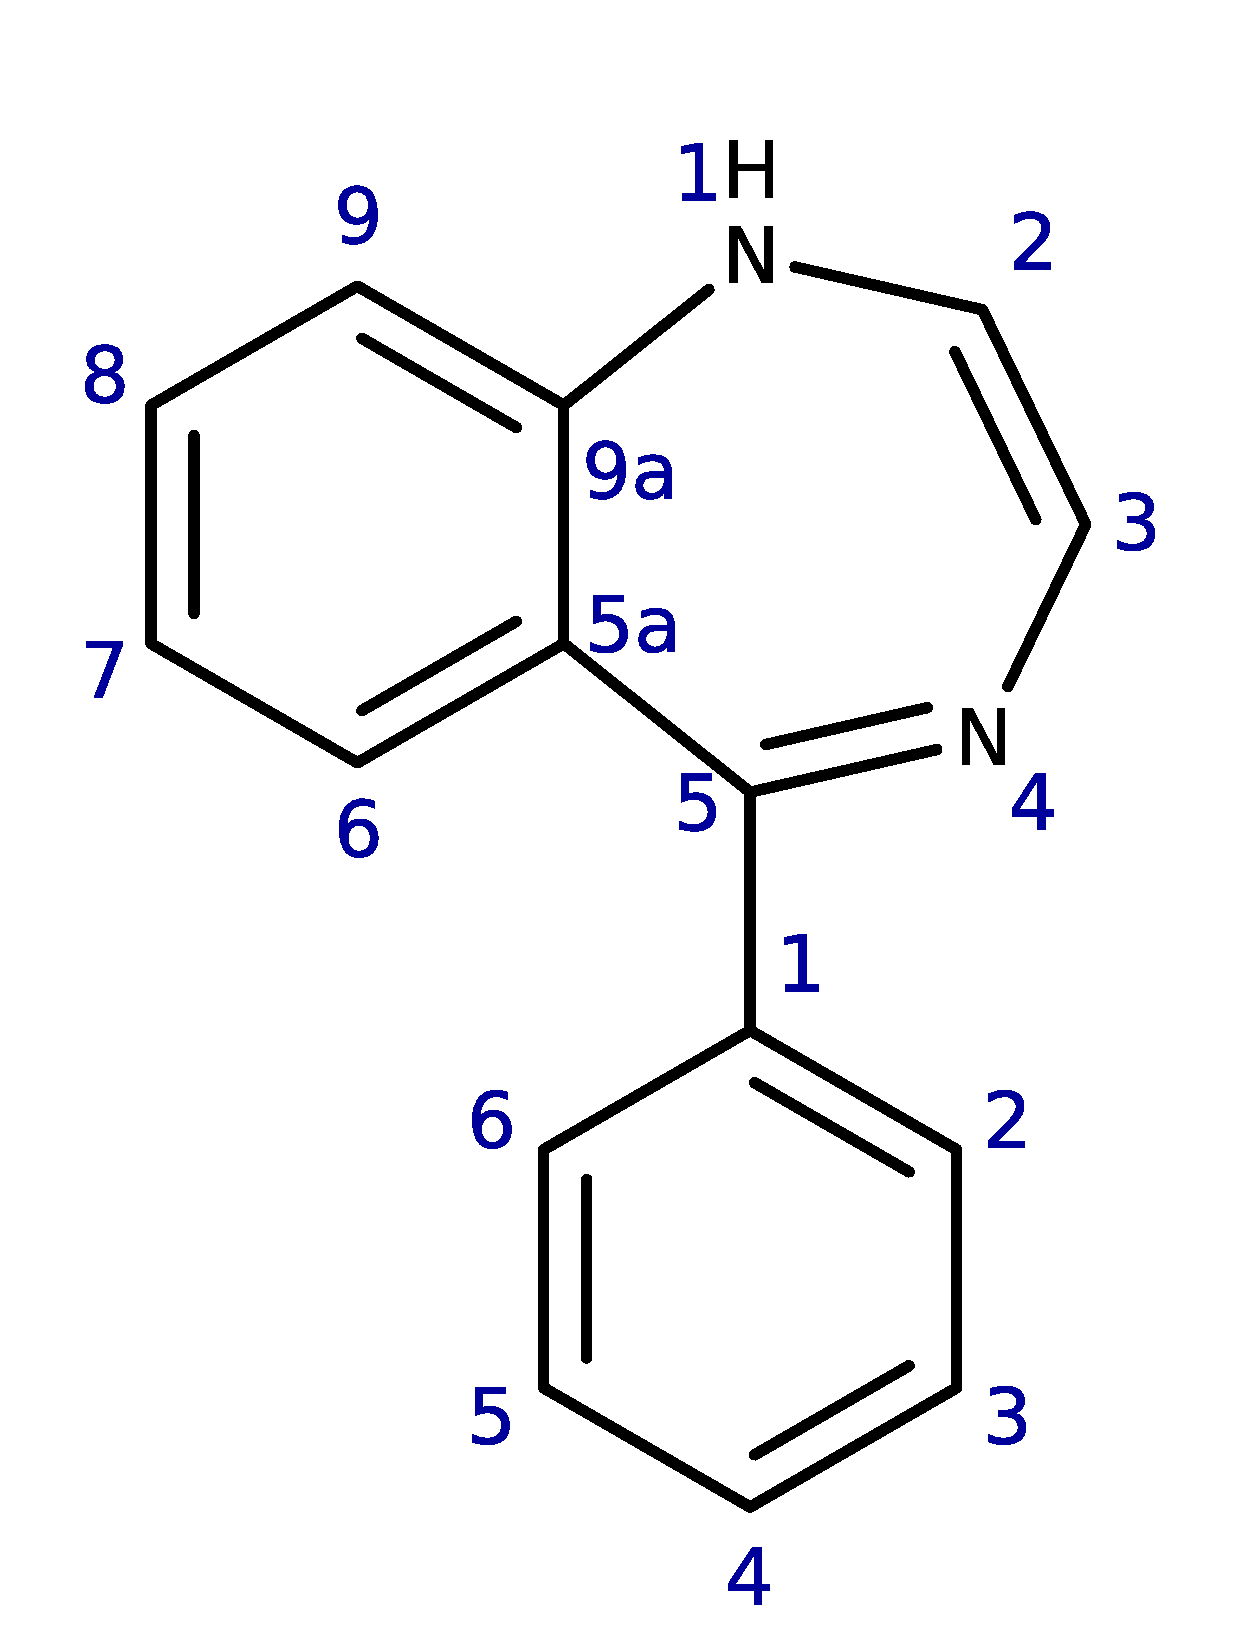
\includegraphics[width=\linewidth]{benzo.jpg}
  \captionof{figure}{The number of deaths resulted from overdosing of benzodiazepines}
  \label{fig:bnz}
\end{minipage}
\end{figure}





\section{Lorazepam} 
Side effects of Lorazepam include
\begin{multicols}{2}
\begin{itemize}
\item Drowsiness
\item Dizziness
\item Tiredness
\item Muscle weakness
\item Headache
\item Blurred vision
\item Sleep problems (insomnia)
\item Loss of balance or coordination
\item Forgetfulness or amnesia
\item Difficulty concentrating
\item Nausea
\item Vomiting
\item Constipation
\item Changes in appetite
\item Skin rash
\end{itemize}
\end{multicols}
Serious side effects. If any of these is present, seek medical attention immediately
\begin{itemize}
\item confusion, depressed mood, thoughts of suicide or hurting yourself.
\item hyperactivity, agitation, hostility.
\item hallucinations.
\item feeling light-headed, fainting.
\end{itemize}